\documentclass{article}
\usepackage[utf8]{inputenc}
\usepackage{mdframed}
\usepackage{amssymb}
\usepackage{abstract}
\usepackage{graphicx}
\renewcommand{\abstractname}{}

\title{An Introduction to Quadratics}
\author{Alexander Chen}

\begin{document}
\maketitle

\begin{abstract}
  I've said it before: equations are the devil's sentences. The worst one is that quadratic equation, an infernal salad of numbers, letters, and symbols.

  \medskip

  ---Stephen Colbert
\end{abstract}


\section{Fundamentals}
Quadratic equations can be found in almost every type of math, and in many math competitions. This section may be review for many of you, so feel free to skip ahead.
\begin{mdframed}
  \textbf{Definition 1.1.} A quadratic equation is a special kind of polynomial that has a degree of 2, which means that it highest power exponent of $x$ is 2.
\end{mdframed}
\begin{mdframed}
  \textbf{Definition 1.2.} The standard form of a quadratic is as follows:
  $$ax^2+bx+c=0$$
\end{mdframed}
\begin{mdframed}
  \textbf{Definition 1.3.} The roots (or zeros) of a quadratic are the values of $x$ such that $ax^2+bx+c=0$.
\end{mdframed}
\begin{mdframed}
  \textbf{Definition 1.4.} The ``leading coefficient" of a quadratic is the coefficient of $x^2$, or $a$.
\end{mdframed}
You will often be required to derive the roots of a quadratic. There are few ways to accomplish this.

\subsection{Factoring}
Factoring is the most common method for finding the roots of a quadratic. The key is to find two numbers whose product equals $a\cdot c$ and whose sum equals $b$, rewrite the quadratic, and then factor. This is best explained with an example. Consider the quadratic: $$2x^2+3x+1$$
We see that $a \cdot c = 2$ and $b = 3$. Two numbers that satisfy this are 1 and 2. Now we rewrite the quadratic as:
$$2x^2+x+2x+1$$
The first two terms can be rewritten as $x(2x+1)$, and the last two terms as $1(2x+1)$. Factor to get:
$$(x+1)(2x+1)$$
Remember, we want to find the values of x such that the above expression equals 0. Since 0 times anything is zero, we can set each term equal to 0. $x+1=0$ gives us $x=-1$ as a root, and $2x+1=0$ gives us $x=-\frac{1}{2}$ as a root.\\\\
\textbf{Note:} In cases where the leading coefficient ($a$) is just 1, we can directly write the final form. Take $x^2+2x+3$. The two numbers whose sum is 2 and product is 3 are clearly 1 and 2. We slap these two numbers on the end of two $(x + \dots)$'s to get $(x+1)(x+2)$. The roots are therefore $x=-1,-2$.
\begin{mdframed}
  \textbf{Exercise 1.5.} Find the roots of $x^2+9x+20$.
\end{mdframed}

\subsection{Completing the Square}
Completing the square is a handy method used not only for factoring but also for many other things. The key is to transform the original quadratic as such:
$$ax^2+bx+c=(x+d)^2+e=0$$
We can use $2x^2+3x+1=0$ as an example again. Divide by two on both sides:
$$x^2+\frac{3}{2}x+\frac{1}{2}=0$$
If one expands $(x+c)^2$, one gets $x^2+2cx+c^2$. We match terms and see that we can rewrite the equation as follows:
$$x^2+2 \cdot \frac{3}{4}x+\frac{9}{16}-\frac{1}{16}=0$$
Then, factor to form the perfect square.
$$(x+\frac{3}{4})^2=\frac{1}{16}$$
We can take the square root of both sides and rearrange, not forgetting the $\pm$. If the right hand side is negative, we can derive the complex roots with $i$.
$$x=\frac{-3\pm1}{16}$$
Then, $x=-\frac{1}{2},-1$.
\begin{mdframed}
  \textbf{Exercise 1.6.} Complete the square and then find the roots of $x^2+6x+7$.
\end{mdframed}

\subsection{The Quadratic Formula}
\begin{mdframed}
  \textbf{Theorem 1.7.} The roots of a quadratic can be expressed as: $$x=\frac{-b\pm\sqrt{b^2-4ac}}{2a}$$
\end{mdframed}
Let's prove this powerful formula. We start with the general quadratic. $$ax^2+bx+c=0$$
Our goal is to complete the square. Divide by $a$ on both sides.
$$x^2+\frac{b}{a}x+\frac{c}{a}=0$$
Adding $(\frac{b}{2a})^2$, or $\frac{b^2}{4a^2}$, to both sides of the equation allows us to complete the square.
$$x^2+\frac{b}{a}x+\frac{b^2}{4a^2}+\frac{c}{a}=\frac{b^2}{4a^2}$$
$$(x+\frac{b}{2a})^2=\frac{b^2}{4a^2}-\frac{c}{a}$$
Equalize the denominators on the right-hand side:
$$(x+\frac{b}{2a})^2=\frac{b^2-4ac}{4a^2}$$\\
We take the square root.
$$x+\frac{b}{2a}=\frac{\pm\sqrt{b^2-4ac}}{2a}$$
Subtracting $\frac{b}{2a}$ gives us our final form:
$$x=\frac{-b\pm\sqrt{b^2-4ac}}{2a}$$
I highly recommend you to memorize this formula if you haven't already; it's incredibly useful.

\subsection{Po-Shen Loh's Quadratic Method}
This final technique, parts of which were known by the ancient Babylonians and Vieta alike, has recently been discovered by USA IMO Coach and Carnegie Mellon Professor Po-Shen Loh.
\\\\Let's consider the quadratic $x^2+4x+5$. If we used the factoring method, we would try to find two numbers whose sum is 4 and whose product is 5. Here, we notice that if the sum of the two numbers is 4, then the sum of the two roots is $-4$, and their average is $-2$. Let's define the two roots as $-2+u$ and $-2-u$. We also know:
$$(-2+u)(-2-u)=5$$
$$4-u^2=5$$
$$u=3$$
Then, the roots are 1 and $5$. Note that we can state $u=3$ W.L.O.G. because plugging in $u=-3$ gives us the same results.

\subsection{Complex Roots}
I'll use a quick example to quickly illustrate how to solve a quadratic with complex roots.
\begin{mdframed}
  \textbf{Example 1.8.} Find the roots of the quadratic $2x^2+6x+18$.
\end{mdframed}
\textit{Solution}. Let's complete the square. First, divide by two on both sides to get: $$x^2+3x+9=0$$
Complete the square.
$$(x+\frac{3}{2})^2+9=\frac{9}{4}$$
$$(x+\frac{3}{2})^2=-\frac{27}{4}$$
Since the right hand side is negative, we know that we will have complex roots.
$$x+\frac{3}{2}=\pm\sqrt{-\frac{27}{4}}$$
Recall that $i^2=-1$. We factor out $\frac{3}{2}i$.
$$x+\frac{3}{2}=\pm\frac{3\sqrt{3}}{2}i$$
Finally,
$$x=-\frac{3}{2}\pm\frac{3\sqrt{3}}{2}i$$

\subsection{Problems}
\textbf{Problem 1.1.} Find the roots of $-x^2-6x-9$.\\\\
\textbf{Problem 1.2.} Find the roots of $x^2+x$.

\section{The Discriminant}
The discriminant is a crucial tool in solving problems related to quadratics, or polynomials of degree two. It also can be useful when dealing with inequalities.\\

Take a look at this equation, derived during our proof of the quadratic formula.
$$(x+\frac{b}{2a})^2=\frac{b^2-4ac}{4a^2}$$\\

\begin{mdframed}
  \textbf{Definition 2.1.} The discriminant of a quadratic in the form $ax^2+bx+c=0$ is the number $b^2-4ac$.
\end{mdframed}

We know that a number $c \in \mathbb{R}$ ($c$ is a real number) has $c^2>0$. However, if $c^2<0$, $c \not\in \mathbb{R}$ ($c$ is a non-real complex number). The left-hand side of the key equation, $(x+\frac{b}{2a})^2$, follows the same rules. Note that since $4a^2 > 0$, the discriminant is the deciding factor for whether $(x+\frac{b}{2a})^2 \in \mathbb{R}$ or not. We get the following theorem:\\

\begin{mdframed}
    \textbf{Theorem 2.2.}
    \begin{itemize}
        \item If the discriminant is less than 0, then $ax^2+bx+c$ does not have real roots.
        \item If the discriminant is equal to 0, then $ax^2+bx+x$ has one real root.
        \item If the discriminant is greater than 0, then $ax^2+bx+c$ has two real roots.
    \end{itemize}
\end{mdframed}

\begin{mdframed}
  \textbf{Exercise 2.3.} Check if $5x^2+6x+8$ has real roots and if so, the number of real roots.
\end{mdframed}
\emph{Solution}. The discriminant of the quadratic equals $6^2-4\cdot8\cdot5 = -124$. Since $-124 < 0$, there are no real roots.

\begin{figure}
  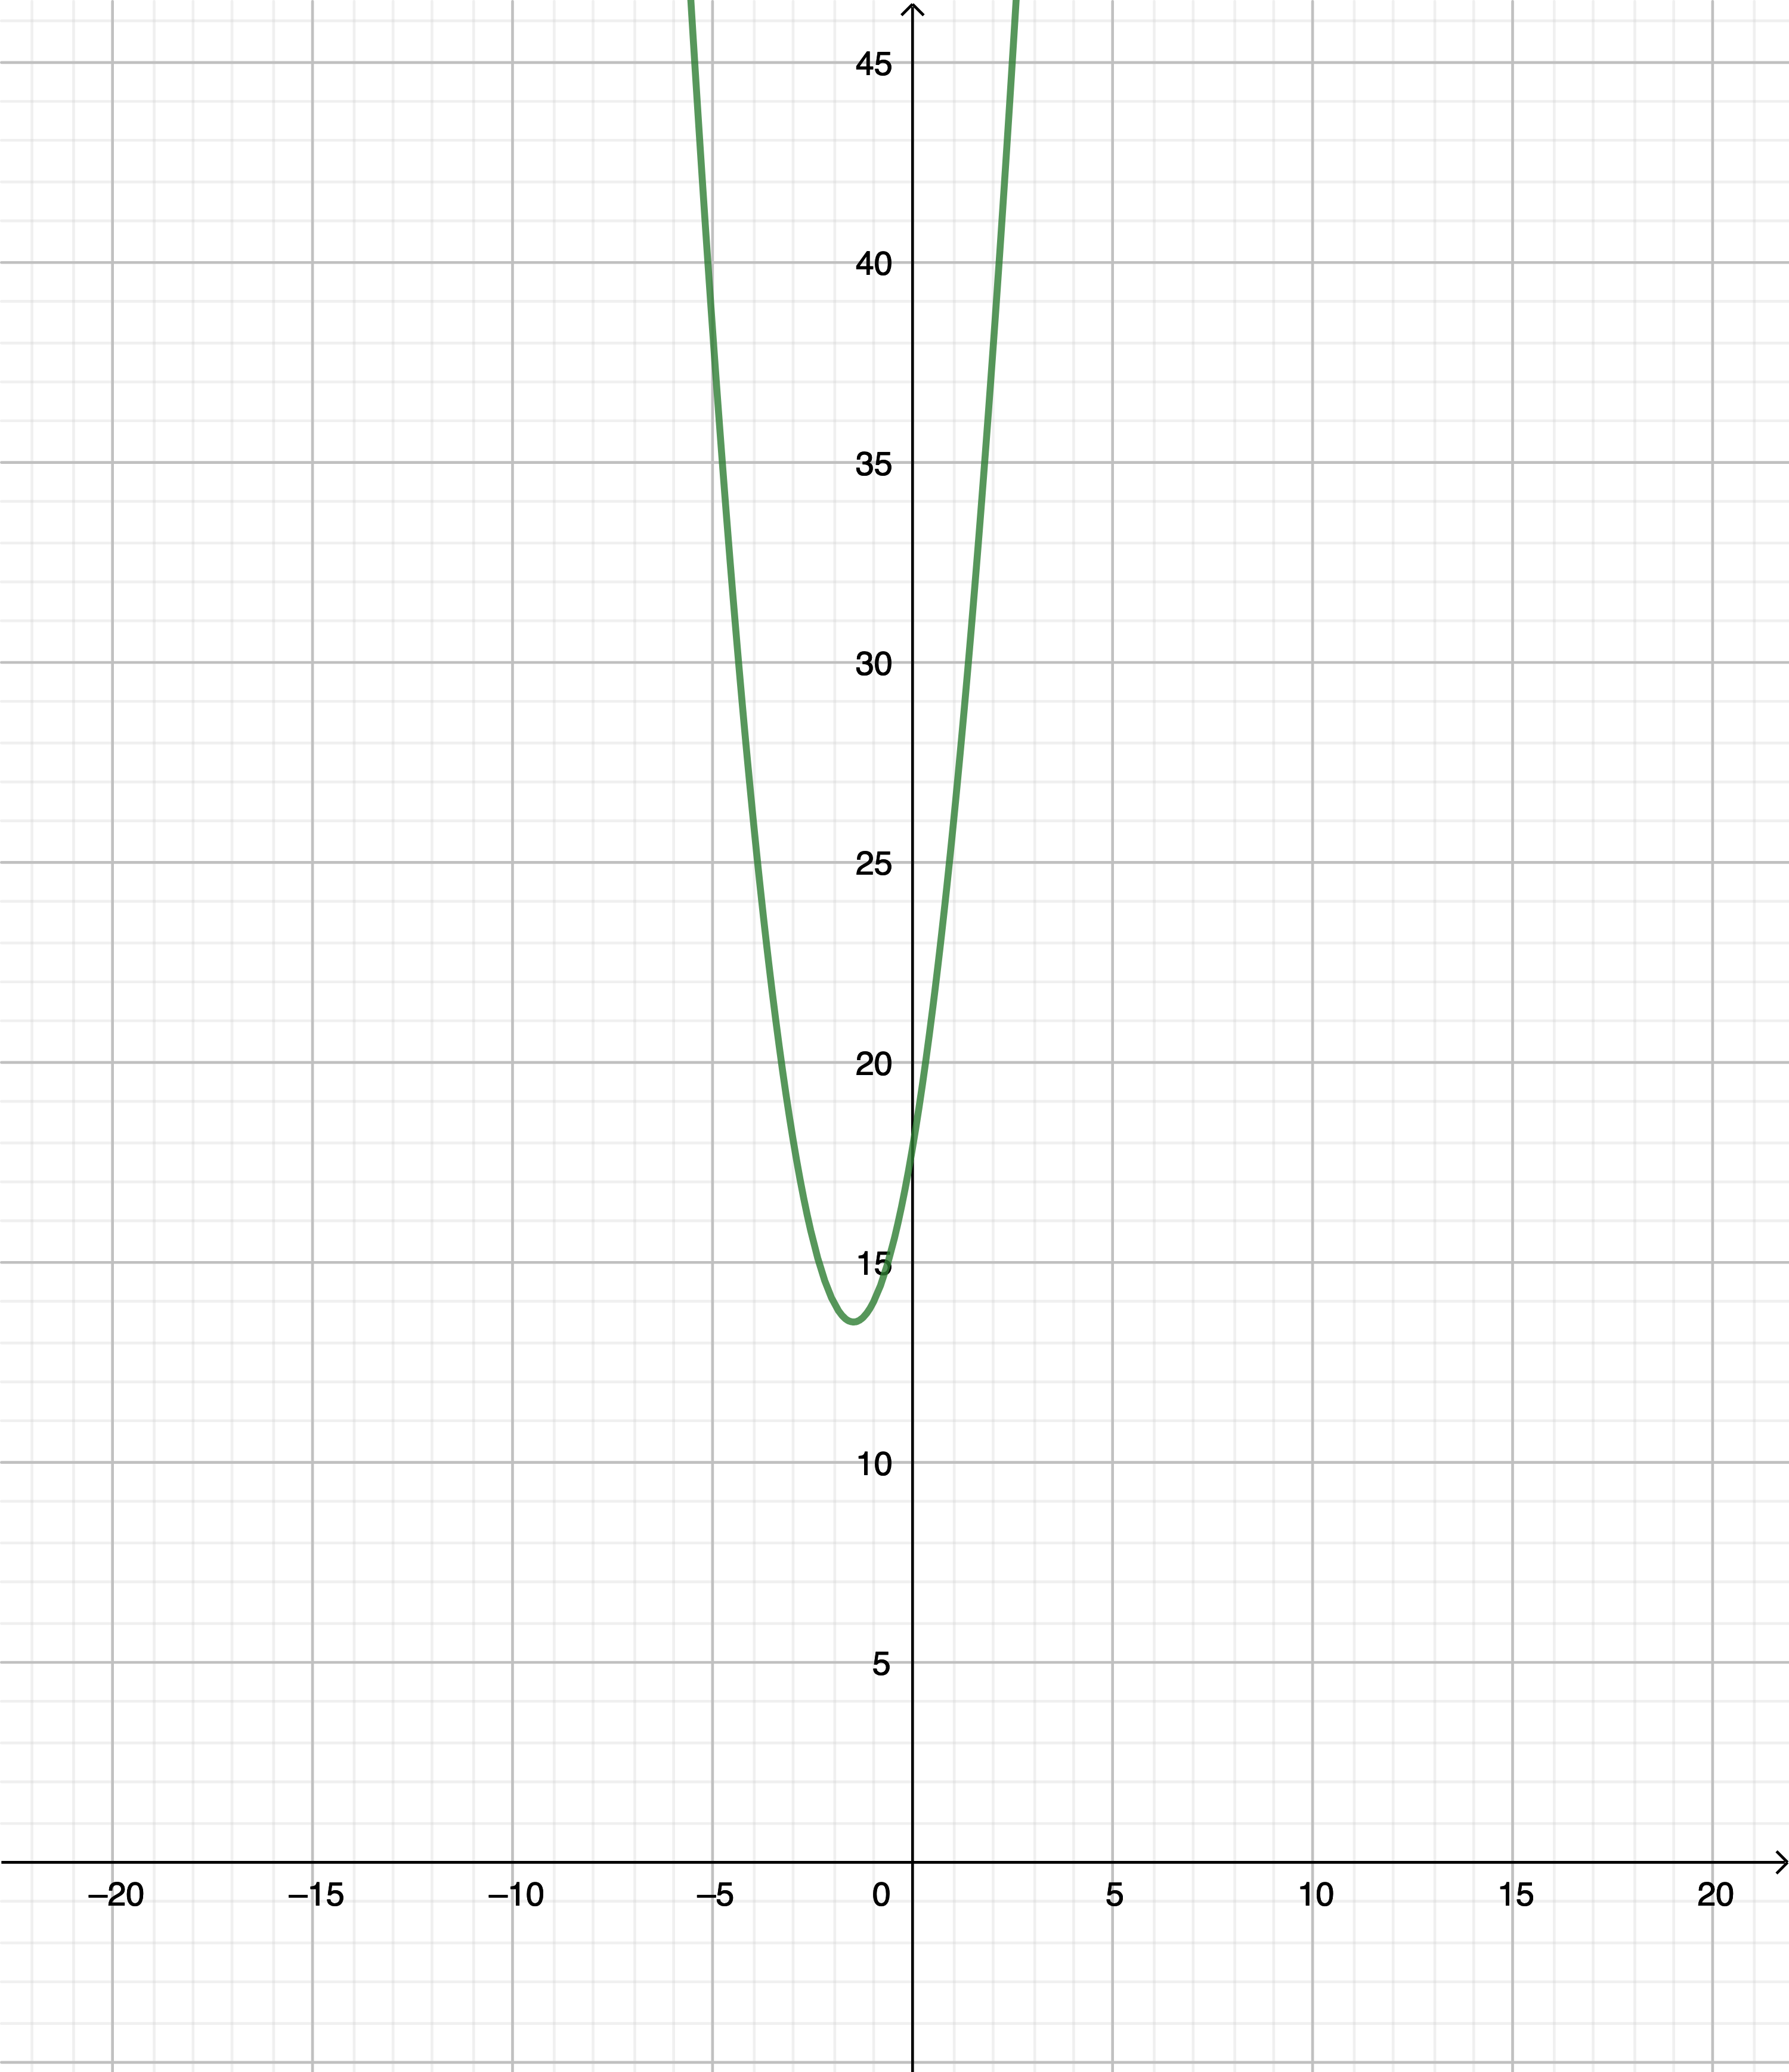
\includegraphics[height=8cm]{intro-to-quadratics-1.png}
  \caption{Graph of $2x^2+6x+18$}
\end{figure}



\end{document}
